\chapter{الأعداد الكمية والتوزيعات الإلكترونية}\label{ch:b1:quantum-numbers}

املأ أنبوبًا زجاجيًا بالهيدروجين تحت ضغط منخفض، ومرِّر فيه تفريغًا
كهربائيًا، ثم انظر إلى توهجه الوردي عبر موشور: لا ينبسط الضوء في قوس
قزح، بل ينقسم إلى أربعة خطوط حادة --- خط أحمر، وخط أزرق مخضرّ، وخطان
بنفسجيان --- ولا شيء بينها. فالجسم الصلب الساخن يضيء بكل أطوال الموجات،
أما ذرة الهيدروجين فلا تصدر إلا بضعة منها. والتفسير، الذي اكتُشف بين
1913 و1926، أن طاقة الإلكترون في الذرة لا تأخذ أي قيمة كانت: إنها
\emph{مكمّاة}. يعرض هذا الفصل قواعد هذا التكميم كما يستعملها الكيميائي
--- أربعة أعداد كمية وثلاث قواعد للملء --- ويستخرج منها \omterm{def:b1:quantum-numbers:configuration}{التوزيع
الإلكتروني} لكل ذرة ولكل أيون، وهو مفتاح الجدول الدوري الذي يدرسه الفصل
التالي.

\begin{recall}
وزّع الكتاب الأول (الصف العاشر) إلكترونات العناصر العشرين الأولى على
الطبقات والطبقات الفرعية 1s و2s و2p و3s و3p، وسمّى إلكترونات الطبقة
الخارجية \omterm{def:b1:quantum-numbers:configuration}{إلكترونات التكافؤ}. ونستعمل من الفيزياء، على أنه معلوم، أن الضوء
الذي طول موجته $\lambda$ مكوَّن من فوتونات طاقتها
$E = h\nu = hc/\lambda$، حيث $h$ ثابت بلانك و$c$
سرعة الضوء.
\end{recall}

\begin{omfigure}

\includegraphics[width=0.62\linewidth]{images/book2/ai/b1-01-street-lamps.jpg}

{\small مصابيح شوارع بالصوديوم تحت ضغط منخفض. ضوؤها يكاد يكون خطًا واحدًا
برتقاليًا مصفرًّا: فذرة الصوديوم المثارة، مثل ذرة الهيدروجين، لا تصدر
إلا فوتونات ذات طاقات محددة قليلة.}
\end{omfigure}

\section{طاقات مكمّاة: طيف الهيدروجين}

\begin{definition}[مستوى الطاقة، الحالة الأساسية، الحالة المثارة]\label{def:b1:quantum-numbers:energy-level}
لا تأخذ طاقة إلكترون مرتبط في ذرة إلا قيمًا معيّنة، هي
\emph{مستويات الطاقة}\index{مستوى طاقة} للذرة. ويؤخذ صفر الطاقة
عندما يكون الإلكترون ساكنًا على بعد لانهائي من النواة (أي عندما تتأين
الذرة)، فيكون كل مستوى لإلكترون مرتبط سالبًا. وأدنى مستوى هو
\emph{الحالة الأساسية}\index{حالة أساسية}؛ وكل مستوى آخر
\emph{حالة مثارة}\index{حالة مثارة}.
\end{definition}

تنتقل الذرة من مستوى طاقته $E_{\text{أعلى}}$ إلى مستوى أدنى
$E_{\text{أدنى}}$ بإصدار فوتون واحد، ومن المستوى الأدنى إلى الأعلى
بامتصاص فوتون واحد، طاقته
\[
  h\nu = \frac{hc}{\lambda} = E_{\text{أعلى}} - E_{\text{أدنى}} .
\]
فطيف الخطوط إذن صورة للفروق بين المستويات.

\begin{theorem}[مستويات طاقة ذرة الهيدروجين]\label{thm:b1:quantum-numbers:levels}
\omterm{def:b1:quantum-numbers:energy-level}{مستويات طاقة} ذرة الهيدروجين هي
\[
  E_n = -\frac{E_R}{n^2}, \qquad n = 1, 2, 3, \dots,
  \qquad E_R = \qty{13.6}{eV},
\]
حيث $E_R$ طاقة ريدبرغ (مصحَّحة بحركة النواة). \omterm{def:b1:quantum-numbers:energy-level}{والحالة الأساسية}
$E_1 = \qty{-13.6}{eV}$، وطاقة تأين الذرة
هي $E_R$.
% ledger: const:RyhcEV, ie:H (13.598 eV; levels computed in
% figdata/bachelor-1/hydrogen-levels.py)
\end{theorem}
\admitted

\begin{remark}[من أين تأتي الصيغة]\label{rem:b1:quantum-numbers:schrodinger}
تنتج الصيغة من حل معادلة شرودنغر للإلكترون في مجال البروتون؛ ويُستخرج
الحل، وأشكال الدوال الموجية التي يعطيها، في مجلد السنة الثانية. وكان
نيلز بور قد حصل على المستويات نفسها سنة 1913 من نموذج أبسط ذي مدارات
دائرية، تُرك اليوم.
\end{remark}

\begin{proposition}[صيغة ريدبرغ]\label{prop:b1:quantum-numbers:rydberg}
تُعطى أطوال موجات الخطوط التي يصدرها الهيدروجين بالعلاقة
\[
  \frac{1}{\lambda} = R_H\left(\frac{1}{n_1^2} - \frac{1}{n_2^2}\right),
  \qquad n_2 > n_1 \ge 1, \qquad R_H = \frac{E_R}{hc},
\]
للانتقال من المستوى $n_2$ نزولًا إلى المستوى $n_1$. والخطوط التي
تنتهي عند المستوى نفسه $n_1$ تكوّن \emph{سلسلة}: سلسلة ليمان من أجل $n_1 = 1$
(فوق البنفسجي)، وسلسلة بالمر من أجل $n_1 = 2$ (المرئي)، وسلسلة باشن من أجل $n_1 = 3$
(تحت الأحمر).
\end{proposition}

\begin{proof}
يحمل الفوتون الطاقة التي فقدتها الذرة:
$hc/\lambda = E_{n_2} - E_{n_1} = -E_R/n_2^2 + E_R/n_1^2
= E_R\,(1/n_1^2 - 1/n_2^2)$. وبالقسمة على $hc$ نحصل على الصيغة.
\end{proof}

\begin{example}[الخط الأحمر للهيدروجين]\label{ex:b1:quantum-numbers:halpha}
من أجل الانتقال $3 \to 2$: $\Delta E = 13.6\,(1/4 - 1/9) =
\qty{1.89}{eV}$. ومع $hc = \qty{1240}{eV.nm}$ (من قيم $h$
و$c$ و$e$)، يكون $\lambda = 1240/1.89 = \qty{656}{nm}$: إنه الخط الأحمر.
وتقع خطوط بالمر الأخرى، $4 \to 2$ و$5 \to 2$ و$6 \to 2$، عند 486
و434 و\qty{410}{nm}؛ أما الخط التالي، $7 \to 2$ عند \qty{397}{nm}،
فهو في فوق البنفسجي. وتتفق الأطوال المقيسة، 656.3 و486.1 و434.0
و\qty{410.2}{nm}، معها بأفضل من جزء من ألفين؛ ويرجع الفرق الصغير
الباقي إلى القياس في الهواء لا في الفراغ.
% ledger: asd:Halpha, asd:Hbeta, asd:Hgamma, asd:Hdelta (computed values
% in figdata/out/bachelor-1-hydrogen-levels-balmer.dat)
\end{example}

\begin{omfigure}
\begin{tikzpicture}
\begin{axis}[
  width=0.62\linewidth, height=7.2cm,
  xmin=0, xmax=10, ymin=-14.5, ymax=0.6,
  axis x line=none, axis y line=left,
  ylabel={\foreignlanguage{arabic}{الطاقة \babelsublr{(eV)}}}, ytick={-14,-12,-10,-8,-6,-4,-2,0},
  tick label style={font=\small}, label style={font=\small},
  clip=false]
\pgfplotsinvokeforeach{-13.598,-3.400,-1.511,-0.850,-0.544}{
  \draw[black!70, line width=0.7pt] (axis cs:0.3,#1) -- (axis cs:9.6,#1);}
\draw[black!40, dashed] (axis cs:0.3,0) -- (axis cs:9.6,0);
\node[font=\small, anchor=west] at (axis cs:9.7,-13.598) {$n = 1$};
\node[font=\small, anchor=west] at (axis cs:9.7,-3.400) {$n = 2$};
\node[font=\small, anchor=west] at (axis cs:9.7,-1.511) {$n = 3$};
\node[font=\small, anchor=south west] at (axis cs:9.7,0.05) {$n \to \infty$};
% Lyman
\draw[-{Stealth}, violet!70!black, thick] (axis cs:1.0,-3.400) -- (axis cs:1.0,-13.598);
\draw[-{Stealth}, violet!70!black, thick] (axis cs:1.6,-1.511) -- (axis cs:1.6,-13.598);
\draw[-{Stealth}, violet!70!black, thick] (axis cs:2.2,-0.850) -- (axis cs:2.2,-13.598);
\node[font=\small, violet!70!black, anchor=west] at (axis cs:2.4,-9) {ليمان};
% Balmer
\draw[-{Stealth}, red!80!black, thick] (axis cs:4.4,-1.511) -- (axis cs:4.4,-3.400);
\draw[-{Stealth}, teal!80!black, thick] (axis cs:5.0,-0.850) -- (axis cs:5.0,-3.400);
\draw[-{Stealth}, blue!80!black, thick] (axis cs:5.6,-0.544) -- (axis cs:5.6,-3.400);
\node[font=\small, anchor=north] at (axis cs:5.0,-3.6) {بالمر};
% Paschen
\draw[-{Stealth}, black!60, thick] (axis cs:7.8,-0.850) -- (axis cs:7.8,-1.511);
\draw[-{Stealth}, black!60, thick] (axis cs:8.4,-0.544) -- (axis cs:8.4,-1.511);
\node[font=\small, anchor=north] at (axis cs:8.1,-1.7) {باشن};
\end{axis}
\end{tikzpicture}

{\small \omterm{def:b1:quantum-numbers:energy-level}{مستويات طاقة} الهيدروجين، $E_n = -\qty{13.6}{eV}/n^2$،
مرسومة بمقياس صحيح (محسوبة من ثابت ريدبرغ)؛ وتتزاحم المستويات $n = 4,
5, \dots$ تحت الصفر. كل سهم فوتون
واحد صادر؛ والأسهم التي تنتهي عند المستوى نفسه تكوّن سلسلة.}
\end{omfigure}

\begin{omfigure}
\begin{tikzpicture}
\begin{axis}[
  width=0.9\linewidth, height=3.0cm,
  xmin=360, xmax=700, ymin=0, ymax=1,
  axis x line=bottom, axis y line=none,
  xlabel={\foreignlanguage{arabic}{طول الموجة \babelsublr{(nm)}}}, xtick={400,450,500,550,600,650,700},
  tick label style={font=\small}, label style={font=\small},
  clip=false]
\fill[black!85] (axis cs:360,0) rectangle (axis cs:700,1);
% line positions: figdata/out/bachelor-1-hydrogen-levels-balmer.dat
\draw[line width=1.6pt, red!90!black] (axis cs:656.5,0) -- (axis cs:656.5,1);
\draw[line width=1.6pt, cyan!80!green] (axis cs:486.3,0) -- (axis cs:486.3,1);
\draw[line width=1.6pt, blue!70!violet] (axis cs:434.2,0) -- (axis cs:434.2,1);
\draw[line width=1.6pt, violet!75] (axis cs:410.3,0) -- (axis cs:410.3,1);
\draw[white, dashed] (axis cs:364.7,0) -- (axis cs:364.7,1);
\node[font=\small, anchor=south] at (axis cs:364.7,1.02) {الحد};
\node[font=\small, anchor=south] at (axis cs:656.5,1.02) {$3\to2$};
\node[font=\small, anchor=south] at (axis cs:486.3,1.02) {$4\to2$};
\node[font=\small, anchor=south] at (axis cs:434.2,1.02) {$5\to2$};
\node[font=\small, anchor=south east] at (axis cs:412,1.02) {$6\to2$};
\end{axis}
\end{tikzpicture}

{\small خطوط بالمر محسوبة من صيغة ريدبرغ (أطوال الموجات في الفراغ)، على
النطاق المرئي. وتتزاحم خطوط أخرى نحو حد السلسلة
عند \qty{364.7}{nm}، في فوق البنفسجي.}
\end{omfigure}

\begin{history}[ذرة بور، 1913]
اقترح نيلز بور سنة 1913، وهو فيزيائي دنماركي في الثامنة والعشرين يعمل في
مانشستر، أن إلكترون الهيدروجين لا يدور حول النواة إلا على مدارات معيّنة،
وأن الضوء يصدر حين يقفز من مدار إلى مدار أدنى. فأعطى نموذجه خطوط بالمر
بدقة، وقيمة ثابت ريدبرغ انطلاقًا من $h$ و$e$ وكتلة الإلكترون. ولم تصمد
المدارات أمام ميكانيك الكم في 1925--1926، لكن المستويات المكمّاة صمدت.
ونال بور جائزة نوبل في الفيزياء سنة 1922.
\end{history}

\begin{omfigure}
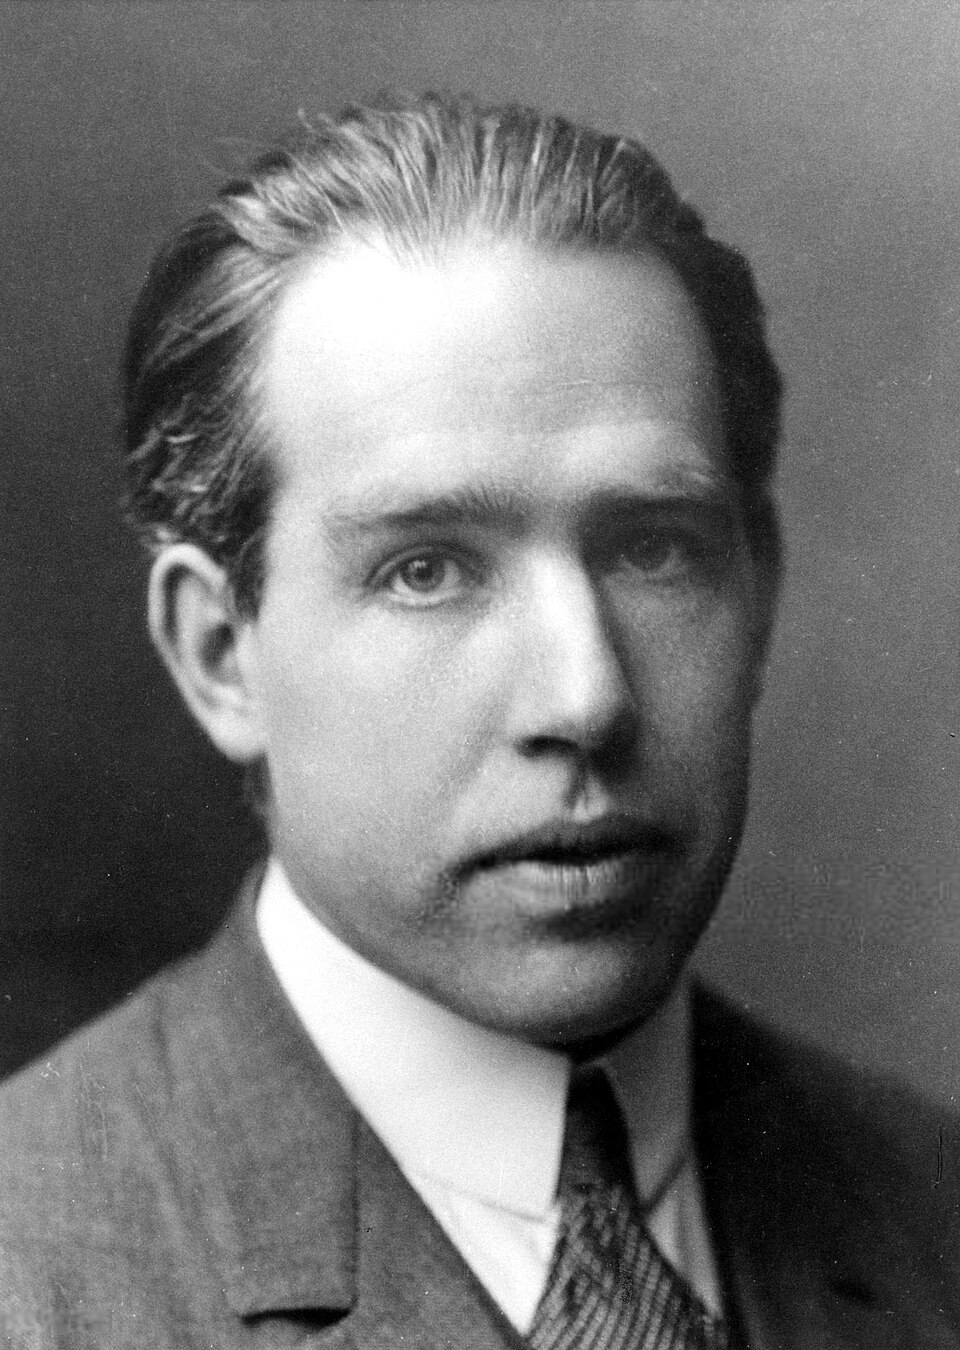
\includegraphics[width=0.26\linewidth]{images/book2/bohr.jpg}

{\small نيلز بور (1885--1962)، نحو سنة 1922.}
\end{omfigure}

\section{أربعة أعداد كمية}

في ذرة متعددة الإلكترونات لا تُعطى الطاقات بصيغة واحدة، لكن كل إلكترون
يبقى موصوفًا بمجموعة صغيرة من الأعداد الصحيحة، هي أعداده الكمية.

\begin{definition}[الأعداد الكمية]\label{def:b1:quantum-numbers:quantum-number}
تُوسم حالة إلكترون في ذرة بأربعة أعداد:
\begin{itemize}
  \item \emph{العدد الكمي الرئيسي}\index{عدد كمي رئيسي}
        $n = 1, 2, 3, \dots$، الذي يحدد أساسًا الطاقة والحجم؛
  \item \emph{العدد الكمي السمتي}\index{عدد كمي سمتي}
        (أو العدد الكمي الثانوي) $l = 0, 1, \dots, n-1$، الذي يحدد
        الشكل؛ ويُكتب $l = 0, 1, 2, 3$ بالحروف s وp وd وf؛
  \item \emph{العدد الكمي المغناطيسي}\index{عدد كمي مغناطيسي}
        $m_l = -l, -l+1, \dots, l$، الذي يحدد الاتجاه ($2l + 1$
        قيمة)؛
  \item \emph{العدد الكمي المغزلي}\index{عدد كمي مغزلي}
        $m_s = +\tfrac12$ أو $-\tfrac12$، وهو خاصية ذاتية
        للإلكترون، يُرسم سهمًا متجهًا إلى الأعلى أو إلى الأسفل.
\end{itemize}
\end{definition}

\begin{definition}[المدار الذري، الطبقة، الطبقة الفرعية]\label{def:b1:quantum-numbers:orbital}
\emph{المدار الذري}\index{مدار ذري} حالة إلكترون واحد موسومة بالأعداد
الثلاثة $(n, l, m_l)$؛ ويُرسم خانةً واحدة،
\omorbs{}. والمدارات التي لها العدد $n$ نفسه تكوّن \emph{طبقة
إلكترونية}\index{طبقة إلكترونية}؛ والتي لها $n$ و$l$ نفساهما تكوّن
\emph{طبقة فرعية}\index{طبقة فرعية}، تُسمّى بالعدد $n$ وبحرف $l$:
فالطبقة 2p هي الطبقة الفرعية $n = 2$، $l = 1$، المكوّنة من ثلاثة مدارات
($m_l = -1, 0, 1$).
\end{definition}

\begin{remark}[الأشكال]\label{rem:b1:quantum-numbers:shapes}
المدار s كروي؛ وللمدار p فصّان على امتداد محور، وتتجه مدارات 2p
الثلاثة على امتداد $x$ و$y$ و$z$. أما الوصف الرياضي لهذه الأشكال
--- الدوال الموجية، وجزآها القطري والزاوي، وعُقدها --- فمكانه مجلد
السنة الثانية. وفي هذا الكتاب، المدار خانة تتسع لإلكترونين على الأكثر.
\end{remark}

\begin{proposition}[سعة الطبقة الفرعية وسعة الطبقة]\label{prop:b1:quantum-numbers:capacity}
تحوي \omterm{def:b1:quantum-numbers:orbital}{الطبقة الفرعية} ذات العدد السمتي $l$ عدد $2l + 1$ من المدارات، وتتسع
لعدد $2(2l + 1)$ من الإلكترونات: 2 في s، و6 في p، و10 في d، و14 في f.
وتحوي الطبقة $n$ عدد $n^2$ من المدارات، وتتسع لعدد $2n^2$ من الإلكترونات.
\end{proposition}

\begin{proof}
من أجل $l$ معطى، يأخذ $m_l$ القيم $2l + 1$ من $-l$ إلى $l$، ويتسع كل
مدار لإلكترونين مغزلاهما متعاكسان (\cref{prop:b1:quantum-numbers:pauli}
أدناه). ومن أجل $n$ معطى، يمتد $l$ من $0$ إلى $n - 1$، فيكون عدد
المدارات
\[
  \sum_{l=0}^{n-1} (2l+1) = 2\,\frac{(n-1)n}{2} + n = n^2 ,
\]
وعدد الإلكترونات $2n^2$: أي 2 و8 و18 و32 من أجل $n = 1$ إلى 4.
\end{proof}

\begin{example}[الطبقة الثالثة]\label{ex:b1:quantum-numbers:third}
من أجل $n = 3$: $l = 0$ (3s، مدار واحد)، و$l = 1$ (3p، ثلاثة مدارات)،
و$l = 2$ (3d، خمسة مدارات، $m_l = -2, \dots, 2$): أي تسعة مدارات وما
يصل إلى 18 إلكترونًا. ولإلكترون في 3d مثلًا الأعداد
الكمية $(3, 2, -1, +\tfrac12)$.
\end{example}

\section{بناء التوزيعات}

\begin{definition}[التوزيع الإلكتروني]\label{def:b1:quantum-numbers:configuration}
\emph{التوزيع الإلكتروني}\index{توزيع إلكتروني} لذرة أو لأيون هو قائمة
طبقاته الفرعية المشغولة مع عدد الإلكترونات في كل منها، مكتوبًا أسًّا:
$1\text{s}^2 2\text{s}^2
2\text{p}^4$ للأكسجين. وإلكترونات أكبر $n$، ومعها إلكترونات \omterm{def:b1:quantum-numbers:orbital}{طبقة فرعية} d
أو f غير ممتلئة، هي \emph{إلكترونات
التكافؤ}\index{إلكترونات التكافؤ}؛ والبقية هي \emph{الإلكترونات
الداخلية}\index{إلكترونات داخلية}. ويُختصر التوزيع بكتابة توزيع الغاز
النبيل السابق بين معقوفين:
فالأكسجين $[\ce{He}]\,2\text{s}^2 2\text{p}^4$.
\end{definition}

تعطي ثلاث قواعد توزيع \omterm{def:b1:quantum-numbers:energy-level}{الحالة الأساسية}.

\begin{proposition}[مبدأ الاستبعاد لباولي]\label{prop:b1:quantum-numbers:pauli}
لا يكون لإلكترونين من الذرة نفسها الأعداد الكمية الأربعة نفسها أبدًا.
ومن ثم يتسع المدار الواحد لإلكترونين على الأكثر، يكون مغزلاهما عندئذ
متعاكسين: \omorbs{ud}.
\end{proposition}
\admitted

\begin{proposition}[قاعدة كليتشكوفسكي]\label{prop:b1:quantum-numbers:klechkowski}
في \omterm{def:b1:quantum-numbers:energy-level}{الحالة الأساسية} لذرة متعادلة، تُملأ الطبقات الفرعية بترتيب
تزايد $n + l$، وعند تساوي $n + l$ بترتيب تزايد
$n$:
\[
  1\text{s},\ 2\text{s},\ 2\text{p},\ 3\text{s},\ 3\text{p},\ 4\text{s},\
  3\text{d},\ 4\text{p},\ 5\text{s},\ 4\text{d},\ 5\text{p},\ 6\text{s},\
  4\text{f},\ 5\text{d},\ 6\text{p},\ 7\text{s},\ 5\text{f},\ 6\text{d},\
  7\text{p}.
\]
\end{proposition}
\admitted

\begin{remark}[قاعدة تجريبية]\label{rem:b1:quantum-numbers:klech-empirical}
قاعدة كليتشكوفسكي (وتسمى أيضًا قاعدة مادلونغ) خلاصة لتوزيعات مرصودة، لا
قانون: فهي تصف الترتيب الذي تمتلئ به الطبقات الفرعية مع تزايد الشحنة
النووية. وفي ذرة متعددة الإلكترونات تتنافر الإلكترونات فيما بينها،
فتتعلق طاقة \omterm{def:b1:quantum-numbers:orbital}{الطبقة الفرعية} بالعدد $l$ وبالعدد $n$ معًا: فإلكترون 4s، الذي
يقضي جزءًا من وقته قرب النواة، ينتهي إلى مستوى أدنى من 3d في البوتاسيوم والكالسيوم.
\end{remark}

\begin{omfigure}
\begin{tikzpicture}[font=\small, x=1.25cm, y=0.72cm]
  \foreach \n in {1,...,7} {
    \foreach \l/\s in {0/s,1/p,2/d,3/f} {
      \pgfmathtruncatemacro\ok{(\l<\n) && (\n+\l<=8)}
      \ifnum\ok=1
        \node[draw=black!50, rounded corners=2pt, minimum width=0.85cm,
          minimum height=0.5cm, fill=white] (s\n\l) at (\l,-\n) {\n\s};
      \fi
    }
  }
  \begin{scope}[on background layer]
  \foreach \la/\na/\lb/\nb in {0/1/0/1, 0/2/0/2, 1/2/0/3, 1/3/0/4, 2/3/0/5,
      2/4/0/6, 3/4/0/7, 3/5/1/7} {
    \draw[-{Stealth}, omDef, thick, opacity=0.8]
      ($(\la,-\na)+(0.5,0.42)$) -- ($(\lb,-\nb)+(-0.5,-0.42)$);
  }
  \end{scope}
  \node[anchor=west, align=left, font=\small] at (4.0,-2.5) {\foreignlanguage{arabic}{اتبع كل سهم،}\\ثم السهم الذي\\على يمينه};
\end{tikzpicture}

{\small مخطط كليتشكوفسكي. تقع الطبقات الفرعية ذات المجموع $n + l$ نفسه
على قطر واحد؛ واتباع الأقطار بالترتيب يعطي ترتيب الملء
1s، 2s، 2p، 3s، 3p، 4s، 3d، 4p، 5s، \dots}
\end{omfigure}

\begin{proposition}[قاعدة هوند]\label{prop:b1:quantum-numbers:hund}
عندما يمكن وضع إلكترونات \omterm{def:b1:quantum-numbers:orbital}{طبقة فرعية} في عدة مدارات لها الطاقة نفسها،
يكون \omterm{def:b1:quantum-numbers:energy-level}{للحالة الأساسية} أكبر عدد من المغازل
\emph{المتوازية}: تشغل الإلكترونات مدارات منفصلة، ومغازلها إلى الأعلى،
قبل أن يمتلئ أي مدار بإلكترونين.
\end{proposition}
\admitted

\begin{definition}[الإلكترون المنفرد]\label{def:b1:quantum-numbers:unpaired}
\emph{الإلكترون المنفرد}\index{إلكترون منفرد} إلكترون وحيد في مداره.
والنوع الكيميائي الذي يحمل إلكترونات منفردة ينجذب إلى المغناطيس (فهو
بارامغناطيسي، وهي خاصية تدرسها الفيزياء).
\end{definition}

\begin{method}[كتابة توزيع الحالة الأساسية]\label{met:b1:quantum-numbers:configuration}
لكتابة توزيع ذرة عددها الذري $Z$:
\begin{enumerate}
  \item ضع $Z$ إلكترونًا في الطبقات الفرعية بترتيب كليتشكوفسكي،
        مالئًا كل \omterm{def:b1:quantum-numbers:orbital}{طبقة فرعية} (2، 6، 10، 14) قبل التي تليها؛
  \item اكتب النتيجة بترتيب تزايد $n$ (مع ضم 3d
        إلى $n = 3$)، واختصرها بقلب الغاز النبيل
        السابق؛
  \item ارسم خانات \omterm{def:b1:quantum-numbers:orbital}{الطبقة الفرعية} الأخيرة غير الممتلئة، وطبّق قاعدة
        هوند لعدّ الإلكترونات المنفردة.
\end{enumerate}
\end{method}

\begin{example}[الكربون، النيتروجين، الأكسجين، الحديد]\label{ex:b1:quantum-numbers:examples}
تعطي الطريقة، من أجل أربع ذرات:
\begin{center}
\begin{tabular}{lllc}
\hline
الذرة & التوزيع & آخر \omterm{def:b1:quantum-numbers:orbital}{طبقة فرعية} & المنفردة \\
\hline
\ce{C} ($Z = 6$) & $[\ce{He}]\,2\text{s}^2 2\text{p}^2$ & 2p: \omorbs{u,u,} & 2 \\
\ce{N} ($Z = 7$) & $[\ce{He}]\,2\text{s}^2 2\text{p}^3$ & 2p: \omorbs{u,u,u} & 3 \\
\ce{O} ($Z = 8$) & $[\ce{He}]\,2\text{s}^2 2\text{p}^4$ & 2p: \omorbs{ud,u,u} & 2 \\
\ce{Fe} ($Z = 26$) & $[\ce{Ar}]\,3\text{d}^6 4\text{s}^2$ & 3d: \omorbs{ud,u,u,u,u} & 4 \\
\hline
\end{tabular}
\end{center}
في الحديد، يملأ ترتيب كليتشكوفسكي \babelsublr{4s ($Z = 19, 20$)} قبل 3d
(من $Z = 21$ إلى 30)؛ ويُكتب التوزيع بوضع 3d أولًا.
% ledger: gs:Fe
\end{example}

\begin{omfigure}
\begin{tikzpicture}[font=\small]
  \begin{scope}
    \node[anchor=west] at (0,2.4) {\ce{N}: $1\text{s}^2 2\text{s}^2 2\text{p}^3$};
    \node at (0.5,1.3) {\omorbs{ud}}; \node[below] at (0.5,0.9) {1s};
    \node at (1.6,1.3) {\omorbs{ud}}; \node[below] at (1.6,0.9) {2s};
    \node at (3.1,1.3) {\omorbs{u,u,u}}; \node[below] at (3.1,0.9) {2p};
  \end{scope}
  \begin{scope}[xshift=6.2cm]
    \node[anchor=west] at (0,2.4) {\ce{Cr}: $[\ce{Ar}]\,3\text{d}^5 4\text{s}^1$};
    \node at (1.6,1.3) {\omorbs{u,u,u,u,u}}; \node[below] at (1.6,0.9) {3d};
    \node at (4.0,1.3) {\omorbs{u}}; \node[below] at (4.0,0.9) {4s};
    \node[anchor=west, text width=5.0cm] at (0,-0.1) {\foreignlanguage{arabic}{المرصود: ستة إلكترونات منفردة، لا $3\text{d}^4 4\text{s}^2$}};
  \end{scope}
\end{tikzpicture}

{\small خانات كمية. كل خانة مدار واحد؛ وكل سهم إلكترون واحد
ومغزله. يتبع النيتروجين قاعدة هوند؛ أما الكروم فأحد
استثناءات \cref{prop:b1:quantum-numbers:exceptions}.}
\end{omfigure}

\section{الأيونات والاستثناءات وشكل الجدول}

\begin{proposition}[توزيعات الأيونات]\label{prop:b1:quantum-numbers:ions}
للأنيون الأحادي الذرة توزيع الذرة مع إضافة الإلكترونات الزائدة في
المواضع التالية من ترتيب كليتشكوفسكي؛ ويفقد كاتيون عنصر من الزمر
الرئيسية إلكترونات أكبر $n$. أما كاتيون الفلز الانتقالي فيفقد إلكترونات
\babelsublr{$n$s} \emph{قبل} إلكترونات
\babelsublr{$(n-1)$d}: فالأيون \ce{Fe^{2+}} توزيعه $[\ce{Ar}]\,3\text{d}^6$
و\ce{Fe^{3+}} توزيعه $[\ce{Ar}]\,3\text{d}^5$، لا $[\ce{Ar}]\,3\text{d}^4
4\text{s}^2$.
% ledger: gs:Fe2+, gs:Fe3+
\end{proposition}
\admitted

\begin{remark}[ترتيب الملء ليس ترتيب الإفراغ]\label{rem:b1:quantum-numbers:order}
تمتلئ 4s قبل 3d في البوتاسيوم والكالسيوم، ومع ذلك تُفرَغ أولًا في
أيونات الفلزات الانتقالية. ولا تناقض في ذلك: فترتيب طاقات الطبقات الفرعية
يتغير مع الشحنة النووية ومع عدد الإلكترونات، وفي ذرة فلز انتقالي أو في
أيونه تقع \omterm{def:b1:quantum-numbers:orbital}{الطبقة الفرعية} 3d تحت 4s. وقاعدة كليتشكوفسكي لا تصف إلا الذرات المتعادلة.
\end{remark}

\begin{proposition}[استثناءان في السلسلة الانتقالية الأولى]\label{prop:b1:quantum-numbers:exceptions}
التوزيعان المرصودان \omterm{def:b1:quantum-numbers:energy-level}{للحالة الأساسية} للكروم والنحاس هما
\[
  \ce{Cr}: [\ce{Ar}]\,3\text{d}^5 4\text{s}^1, \qquad
  \ce{Cu}: [\ce{Ar}]\,3\text{d}^{10} 4\text{s}^1 ,
\]
بدلًا من $3\text{d}^4 4\text{s}^2$ و$3\text{d}^9 4\text{s}^2$
اللذين تتنبأ بهما قاعدة كليتشكوفسكي: \omterm{def:b1:quantum-numbers:orbital}{فالطبقة الفرعية} d نصف الممتلئة أو
الممتلئة مستقرة على نحو خاص، والمستويان 4s و3d متقاربان.
% ledger: gs:Cr, gs:Cu
\end{proposition}

\begin{example}[النحاس وأيوناته]\label{ex:b1:quantum-numbers:copper}
توزيع \ce{Cu} هو $[\ce{Ar}]\,3\text{d}^{10} 4\text{s}^1$؛ وتوزيع \ce{Cu+}
$[\ce{Ar}]\,3\text{d}^{10}$، بلا \omterm{def:b1:quantum-numbers:unpaired}{إلكترون منفرد}؛ وتوزيع \ce{Cu^{2+}}
$[\ce{Ar}]\,3\text{d}^9$، \omterm{def:b1:quantum-numbers:unpaired}{بإلكترون منفرد} واحد. أما \ce{Zn^{2+}}، $[\ce{Ar}]\,3\text{d}^{10}$،
فليس له أي \omterm{def:b1:quantum-numbers:unpaired}{إلكترون منفرد}.
% ledger: gs:Cu+, gs:Cu2+, gs:Zn2+
\end{example}

\begin{proposition}[التوزيعات والجدول الدوري]\label{prop:b1:quantum-numbers:table}
تبدأ الدورة $n$ من الجدول الدوري بملء \babelsublr{$n$s} وتنتهي
بملء \babelsublr{$n$p}. والطبقات الفرعية التي تمتلئ بينهما هي، وفق
قاعدة كليتشكوفسكي، \babelsublr{$(n-2)$f} و\babelsublr{$(n-1)$d}. ولذلك تضم الدورات
$2, 8, 8, 18, 18, 32, 32$ عنصرًا، وللغازات النبيلة $Z = 2, 10,
18, 36, 54, 86, 118$.
\end{proposition}

\begin{proof}
لا تحوي الدورات 1 إلى 3 إلا \babelsublr{$n$s} (و\babelsublr{$n$p} من أجل $n \ge 2$): $2$، ثم
$2 + 6 = 8$ مرتين. وفي الدورتين 4 و5 تُضاف \babelsublr{$(n-1)$d}: $2 + 10 + 6 =
18$. وفي الدورتين 6 و7 تُضاف \babelsublr{$(n-2)$f} أيضًا: $2 + 14 + 10 + 6 = 32$. وتُغلق
الغازات النبيلة كل دورة: $2$، $2 + 8 = 10$، $18$، $18 + 18 = 36$،
$54$، $54 + 32 = 86$، $118$.
\end{proof}

\begin{omfigure}
\omperiodictable[colour=blocks, legend]

{\small الجدول الدوري ملوّنًا بحسب آخر \omterm{def:b1:quantum-numbers:orbital}{طبقة فرعية} تمتلئ:
الفئات s وp وd وf. وعرض كل فئة هو سعة طبقتها
الفرعية، 2 و6 و10 و14.}
\end{omfigure}

\section{تمارين}

\begin{exercise}[$\star$]\label{exo:b1:quantum-numbers:1}
أي هذه المجموعات $(n, l, m_l, m_s)$ يمكن أن تصف إلكترونًا في
ذرة؟ علّل كل رفض.
(أ) $(2, 2, 0, +\tfrac12)$؛ (ب) $(3, 1, -1, -\tfrac12)$؛
(ج) $(1, 0, 0, 0)$؛ (د) $(4, 3, -3, +\tfrac12)$؛ (ه) $(3, 0, 1, -\tfrac12)$.
\end{exercise}

\begin{exercise}[$\star$]\label{exo:b1:quantum-numbers:2}
كم مدارًا، وكم إلكترونًا على الأكثر، في الطبقات
الفرعية 3d و4f و5p، وفي الطبقة $n = 2$؟
\end{exercise}

\begin{exercise}[$\star$]\label{exo:b1:quantum-numbers:3}
اكتب توزيعات \omterm{def:b1:quantum-numbers:energy-level}{الحالة الأساسية} للذرات \ce{O} و\ce{P} و\ce{K} و\ce{Ca}
و\ce{Br} ($Z = 8, 15, 19, 20, 35$)، كاملةً ومختصرةً، وأعطِ
عدد \omterm{def:b1:quantum-numbers:configuration}{إلكترونات التكافؤ} لكل منها.
\end{exercise}

\begin{exercise}[$\star$]\label{exo:b1:quantum-numbers:4}
ارسم الخانات الكمية لطبقات التكافؤ الفرعية للنيتروجين والكبريت
والكلور، وعُدّ إلكتروناتها المنفردة.
\end{exercise}

\begin{exercise}[$\star\star$]\label{exo:b1:quantum-numbers:5}
أعطِ توزيعات \ce{Na+} و\ce{Mg^{2+}} و\ce{Al^{3+}} و\ce{F-}
و\ce{O^{2-}} و\ce{Cl-} و\ce{S^{2-}} و\ce{Ca^{2+}}. ومع أي غاز نبيل
يتساوى كل منها في عدد الإلكترونات؟
\end{exercise}

\begin{exercise}[$\star\star$]\label{exo:b1:quantum-numbers:6}
اكتب توزيعات \ce{Ti^{2+}} و\ce{Mn^{2+}} و\ce{Co^{2+}}
و\ce{Ni^{2+}} و\ce{Zn^{2+}} ($Z = 22, 25, 27, 28, 30$) وأعطِ
عدد الإلكترونات المنفردة لكل منها.
\end{exercise}

\begin{exercise}[$\star\star$]\label{exo:b1:quantum-numbers:7}
احسب طاقة الفوتون الصادر وطول موجته في الانتقال
$4 \to 3$ للهيدروجين. في أي جزء من الطيف يقع؟
خذ $E_R = \qty{13.6}{eV}$ و$hc = \qty{1240}{eV.nm}$.
\end{exercise}

\begin{exercise}[$\star\star$]\label{exo:b1:quantum-numbers:8}
عيّن العناصر التي تنتهي توزيعات حالتها الأساسية بما يلي:
(أ) $3\text{s}^2 3\text{p}^4$؛ (ب) $4\text{s}^2 3\text{d}^{10} 4\text{p}^5$؛
(ج) $5\text{s}^1$؛ (د) $4\text{s}^2 3\text{d}^3$. وأعطِ الأعداد الكمية
الأربعة لإلكترون من \omterm{def:b1:quantum-numbers:orbital}{الطبقة الفرعية} الأخيرة في (أ).
\end{exercise}

\begin{exercise}[$\star\star$]\label{exo:b1:quantum-numbers:9}
باستعمال قاعدة كليتشكوفسكي، فسّر لماذا يدخل الإلكترون التاسع عشر
للبوتاسيوم في 4s لا في 3d، ولماذا تضم الدورة 3 ثمانية عناصر
لا ثمانية عشر.
\end{exercise}

\begin{exercise}[$\star\star\star$]\label{exo:b1:quantum-numbers:10}
لأيون ذي إلكترون واحد ونواة شحنتها $Ze$ مستويات
$E_n = -Z^2 E_R/n^2$ (مقبولة دون برهان). من أجل \ce{He+} ($Z = 2$)، احسب
طاقة التأين وطول موجة الانتقال $2 \to 1$.
وقارن بالهيدروجين.
\end{exercise}

\begin{exercise}[$\star\star\star$]\label{exo:b1:quantum-numbers:11}
بيّن هل كل توزيع \omterm{def:b1:quantum-numbers:energy-level}{حالة أساسية} أم \omterm{def:b1:quantum-numbers:energy-level}{حالة مثارة} أم مستحيل، ولماذا: (أ) $1\text{s}^2 2\text{s}^1 2\text{p}^1$؛
(ب) $1\text{s}^2 2\text{s}^2 2\text{p}^7$؛ (ج) $1\text{s}^2 2\text{p}^2$؛
(د) $[\ce{Ne}]\,3\text{s}^2 3\text{p}^3$؛ (ه) $1\text{s}^3$.
\end{exercise}

\begin{exercise}[$\star\star\star$]\label{exo:b1:quantum-numbers:12}
تنجذب أملاح الحديد(III) إلى المغناطيس أكثر من أملاح الحديد(II)،
ولا تنجذب أملاح الزنك أبدًا. رتّب \ce{Fe^{2+}} و\ce{Fe^{3+}}
و\ce{Mn^{2+}} و\ce{Cu^{2+}} و\ce{Zn^{2+}} بحسب عدد إلكتروناتها
المنفردة، وفسّر الملاحظة، بافتراض أن الانجذاب يزداد
مع هذا العدد.
\end{exercise}

\section{مسألة: خطوط مصباح، وعالم بثلاثة مغازل}

\begin{problem}[{مسألة نهاية الأسبوع --- من الخطوط الأربعة لمصباح
هيدروجين إلى أطوال الدورات، وكيف يبدو الجدول لو كان
للإلكترون ثلاث حالات مغزلية}]
\label{pb:b1:quantum-numbers:1}
خذ $E_R = \qty{13.6}{eV}$ و$hc = \qty{1240}{eV.nm}$ في المسألة كلها.
ويمتد النطاق المرئي من نحو 400 إلى \qty{700}{nm}.

\medskip
\noindent\textbf{الجزء الأول --- مصباح الهيدروجين.}
\begin{enumerate}
  \item احسب الطاقات $E_1$ إلى $E_4$ لذرة الهيدروجين.
  \item احسب طاقة الفوتون الصادر وطول موجته في
        الانتقال $3 \to 2$. ما لونه؟
  \item احسب أطوال موجات الانتقالات $4 \to 2$ و$5 \to 2$
        و$6 \to 2$.
  \item لماذا يُظهر مصباح الهيدروجين أربعة خطوط مرئية بالضبط؟
        احسب طول موجة $7 \to 2$ لتدعم الجواب.
  \item احسب حد سلسلة بالمر.
  \item احسب طول موجة أول خط في سلسلة ليمان، $2 \to 1$. لماذا لا
        يمكن رؤيته؟
  \item ما أطول طول موجة لفوتون قادر على تأيين ذرة
        هيدروجين في حالتها الأساسية؟
\end{enumerate}

\medskip
\noindent\textbf{الجزء الثاني --- عدّ الحالات.}
\begin{enumerate}[resume]
  \item عدّد قيم $l$ و$m_l$ من أجل $n = 3$؛ كم مدارًا
        تضم الطبقة؟
  \item بيّن أن الطبقة $n$ تتسع لعدد $2n^2$ من الإلكترونات؛ وطبّق ذلك على $n = 4$.
  \item اكتب ترتيب كليتشكوفسكي حتى 7p.
  \item استنتج أطوال الدورات السبع.
  \item فسّر لماذا لا تظهر \omterm{def:b1:quantum-numbers:orbital}{الطبقة الفرعية} 3d في الدورة 3.
  \item استنتج الأعداد الذرية للغازات النبيلة.
\end{enumerate}

\medskip
\noindent\textbf{الجزء الثالث --- الفلزات الانتقالية.}
\begin{enumerate}[resume]
  \item اكتب توزيع الحديد ($Z = 26$) وارسم خانات 3d
        الخاصة به. كم إلكترونًا منفردًا فيه؟
  \item الأسئلة نفسها من أجل \ce{Fe^{2+}} و\ce{Fe^{3+}}. أي الاثنين
        له \omterm{def:b1:quantum-numbers:orbital}{طبقة فرعية} نصف ممتلئة؟
  \item التوزيع المرصود للكروم هو $[\ce{Ar}]\,3\text{d}^5
        4\text{s}^1$. قارنه بالتوزيع المتوقَّع، وعُدّ الإلكترونات
        المنفردة في كل منهما.
  \item أعطِ توزيعات \ce{Cu} و\ce{Cu+} و\ce{Cu^{2+}}.
  \item أي الأيونين \ce{Cu+} و\ce{Cu^{2+}} له إلكترونات منفردة؟
  \item من بين \ce{Sc^{3+}} و\ce{Ti^{3+}} و\ce{Mn^{2+}} ($Z = 21, 22, 25$)،
        أيها له أكبر عدد من الإلكترونات المنفردة؟
\end{enumerate}

\medskip
\noindent\textbf{الجزء الرابع --- عالم بثلاثة مغازل.}
تخيّل كونًا تخضع فيه $n$ و$l$ و$m_l$ للقواعد نفسها التي تخضع لها في
كوننا، ويبقى فيه ترتيب كليتشكوفسكي على حاله، ويصح مبدأ الاستبعاد،
لكن العدد المغزلي $m_s$ يمكن أن يأخذ ثلاث قيم.
\begin{enumerate}[resume]
  \item كم إلكترونًا يتسع له مدار واحد؟ \omterm{def:b1:quantum-numbers:orbital}{وطبقة فرعية} عددها
        $l$؟ وطبقة $n$؟
  \item أعطِ سعات 1s و2s و2p و3s و3p.
  \item يُغلق الغاز النبيل دورةً \omterm{def:b1:quantum-numbers:orbital}{بطبقة فرعية} p ممتلئة (أو 1s في
        الدورة الأولى). ما العدد الذري لأول غاز نبيل؟
  \item أي عدد ذري يسلك سلوك فلز قلوي، أي بإلكترون
        واحد زائد على الغاز النبيل الأول؟
  \item كم عنصرًا تضم الدورة الثانية؟
  \item احسب العدد الذري للغاز النبيل الثاني في هذا العالم.
\end{enumerate}
\end{problem}
